
\section*{CHƯƠNG 1. THIẾT KẾ KIẾN TRÚC HỆ THỐNG }
\setcounter{section}{1}
\setcounter{subsection}{0} %LƯU Ý MỖI LẦN THÊM CHƯƠNG MỚI CẦN THÊM CÂU NÀY ĐỂ RESET THỨ TỰ CỦA SUBSECTON VỀ 1
\setcounter{table}{0} % LƯU Ý SAU MỖI LẦN GỌI BẢNG HAY HÌNH ẢNH PHẢI THÊM CÂU NÀY ĐỂ RESET THỨ TỰ
\setcounter{figure}{0} %% LƯU Ý SAU MỖI LẦN GỌI BẢNG HAY HÌNH ẢNH PHẢI THÊM CÂU NÀY ĐỂ RESET THỨ TỰ
\addcontentsline{toc}{section}
% \addcontentsline{toc}{section}
{\numberline{}CHƯƠNG 1. THIẾT KẾ KIẾN TRÚC HỆ THỐNG}
Trong chương này, chúng em sẽ tiến hành phân tích hệ thống cho dự án đề tài "Hệ thống quản lý ECG". 
Đây là một hệ thống được thiết kế để quản lý và xử lý dữ liệu điện tâm đồ (ECG) của người dùng. 
Hệ thống cung cấp khả năng ghi lại và hiển thị dữ liệu điện tim, cho phép người dùng theo dõi và 
đánh giá sự hoạt động của tim. 
Người dụng cũng có thể thực hiện trao đổi dựa trên các kết quả điện tim đo được. 
Những thông tin này có thể hữu ích trong việc theo dõi sức khỏe tim mạch, theo dõi hiệu quả của liệu pháp 
và hỗ trợ quyết định của người dùng.



\subsection{Yêu cầu hệ thống}
\subsubsection{Yêu cầu về người dùng hệ thống}
Hệ thống được thiết kế để phục vụ các đối tượng sau:
\begin{itemize}
    \item Bệnh nhân: Người sử dụng hệ thống để thực hiện kiểm tra ECG thông qua Bluetooth và theo dõi sức khỏe của mình. Bệnh nhân có quyền truy cập vào kết quả ECG của mình, được một bác sĩ theo dõi và có thể theo dõi các thông tin liên quan đến điện tim và sức khoẻ.
    \item Bác sĩ: Người sử dụng hệ thống để xem và đánh giá kết quả ECG của bệnh nhân, đưa ra nhận xét và đề xuất điều trị. Bác sĩ có thể trao đổi với bệnh nhân và gửi thông báo quan trọng liên quan đến chăm sóc sức khỏe.
    \item Quản trị viên: Người sử dụng hệ thống để quản lý các tài khoản người dùng, phân công bệnh nhân cho bác sĩ và quản lý mối quan hệ giữa bác sĩ và bệnh nhân.
\end{itemize}

\subsubsection{Yêu cầu chức năng}
Các chức năng chính của hệ thống bao gồm: 
\begin{adjustwidth}{2em}{}
  \begin{itemize}
      \item Ghi lại dữ liệu điện tim: Hệ thống cho phép ghi lại tín hiệu điện tim từ máy đo ECG (Electrocardiogram) hay thiết bị đo điện tim khác. Dữ liệu được chuyển tới ứng dụng của người dùng thông qua Bluetooth để lưu trữ, phân tích và có thể xem lại sau này.
  
      \item Hiển thị và phân tích dữ liệu: Hệ thống hiển thị dữ liệu điện tim theo dạng đồ thị. Hệ thống cũng hỗ trợ xuất ra các tệp đã được chuẩn hoá cho các dữ liệu chuỗi thời gian (time-series database) để phục vụ mục đích phân tích và nghiên cứu sâu hơn.
  
      \item Lưu trữ: Hệ thống hỗ trợ lưu dữ liệu mà người dùng đo được từ thiết bị trên cả ứng dụng và trên server của hệ thống. Dữ liệu điện tim cũng được đồng bộ hóa và lưu trữ trên máy chủ của hệ thống. Qua quá trình đồng bộ hóa, dữ liệu từ ứng dụng được truyền đến máy chủ và được lưu trữ an toàn và bảo mật trên hệ thống. Việc lưu trữ dữ liệu điện tim trên cả ứng dụng và máy chủ giúp đảm bảo rằng dữ liệu quan trọng này được lưu trữ một cách đáng tin cậy và có sẵn cho phân tích hoặc sử dụng tương lai.
  
      \item Trao đổi và chia sẻ thông tin về dữ liệu điện tim: Hệ thống giúp người dùng có thể trao đổi trực tiếp với nhau, chia sẻ kết quả đo điện tim, hỏi đáp về các vấn đề sức khỏe hoặc thảo luận về các quyết định. Điều này mang lại sự tiện lợi và hỗ trợ đáng kể cho người dùng trong việc xác định về tình trạng sức khoẻ hiện tại của bản thân.
  \end{itemize}
  \end{adjustwidth}
  
  

  
  
Hệ thống hỗ trợ các chức năng cơ bản sau đối với người dùng:

Đối với người dùng là bệnh nhân:
\begin{itemize}
    \item Đăng nhập và đăng ký tài khoản bằng thông tin cá nhân, bao gồm tên, địa chỉ email, ngày sinh, số điện thoại và mật khẩu.
    \item Cập nhật các thông tin cá nhân.
    \item Xem kết quả ECG của mình, bao gồm biểu đồ và các thông số liên quan.
    \item Theo dõi các tin tức liên quan đến sức khoẻ và tim mạch.
    \item Nhận thông báo và có thể trao đổi trực tiếp với bác sĩ về tình hình sức khoẻ và các kết quả đo được từ thiết bị.
\end{itemize}

Đối với người dùng là bác sĩ:

\begin{itemize}
    \item Được cấp tài khoản để sử dụng hệ thống.
    \item Cập nhật các thông tin cá nhân.
    \item Xem danh sách bệnh nhân được phân công cho mình và xem kết quả ECG của từng bệnh nhân.
    \item Đánh giá và đưa ra nhận xét về kết quả ECG của bệnh nhân.
    \item Trao đổi các thông tin liên quan đến tình hình sức khoẻ và kết quả đo của bệnh nhân.
\end{itemize}

Đối với người dùng là quản trị viên:
\begin{itemize}
    \item Đăng nhập và đăng ký tài khoản bằng thông tin cá nhân, bao gồm tên, địa chỉ email, số điện thoại và mật khẩu.
    \item Cập nhật thông tin cá nhân.
    \item Quản lý danh sách người dùng trong hệ thống, bao gồm bệnh nhân và bác sĩ.
    \item Phân công bệnh nhân cho các bác sĩ và quản lý mối quan hệ giữa bác sĩ và bệnh nhân.
    \item Quản lý các tin tức được đăng trên ứng dụng của người dùng.
\end{itemize}

\subsubsection{Yêu cầu phi chức năng}
\begin{itemize}
    \item Hệ thống hỗ trợ ngôn ngữ Tiếng Việt và Tiếng Anh.
    \item Hệ thống cần đảm bảo tính bảo mật và quyền riêng tư thông tin của người dùng.
    \item Hệ thống phải có giao diện người dùng thân thiện, dễ sử dụng và có thể tương tác trên các thiết bị di động.
    \item Thời gian phản hồi của hệ thống phải nhanh chóng và ổn định.
    \item Hệ thống cần sao lưu dữ liệu định kỳ để đảm bảo tính an toàn và khả năng khôi phục dữ liệu khi cần thiết.
\end{itemize}

Thông qua việc phân tích yêu cầu hệ thống, chúng ta có cái nhìn tổng quan về các chức năng, yêu cầu phi chức năng và các đối tượng người dùng mà hệ thống phải hỗ trợ. Phần phân tích này sẽ cung cấp cơ sở cho việc thiết kế và phát triển hệ thống quản lý ECG, đáp ứng đầy đủ các yêu cầu của người dùng và đảm bảo hiệu suất, bảo mật và tính khả dụng của hệ thống.
\subsection{Phân tích tổng quan hệ thống}



\subsubsection{Sơ đồ use case}

\paragraph{Use case xem/nhận tin nhắn}
\mbox{}

  \begin{figure}[H]
    \centering
    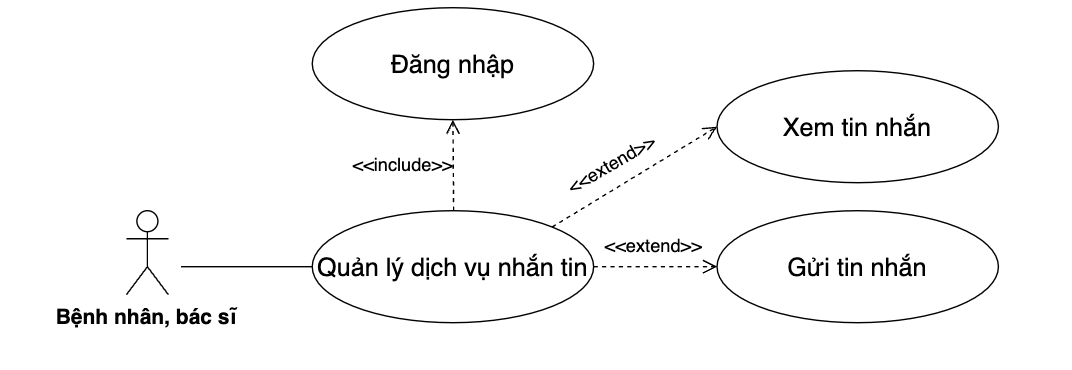
\includegraphics[width=15cm,height=6cm]{Images/mobile_app/use_case_send_receive_message.png}
    \caption[Sơ đồ tuần tự chức năng đăng ký trên App]{\bfseries \fontsize{12pt}{0pt}
    \selectfont Sơ đồ tuần tự chức năng đăng ký trên App}
    \label{hinh21} %đặt tên cho ảnh
  \end{figure}

  \begin{figure}[H]
    \centering
    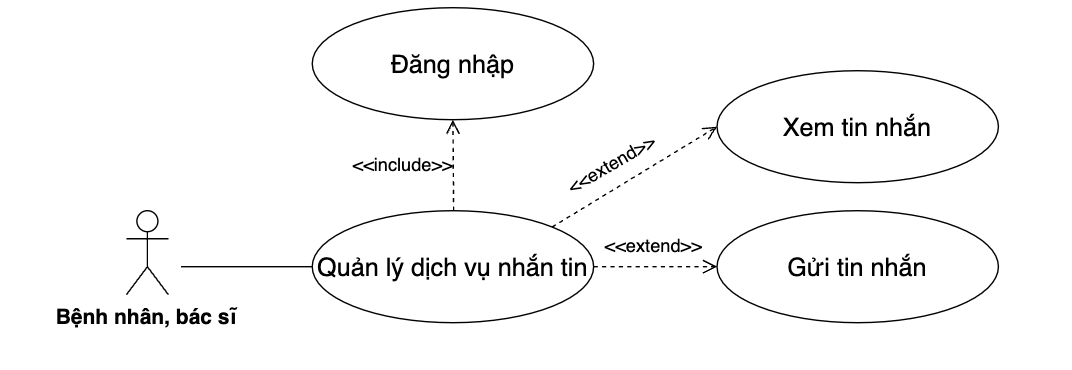
\includegraphics[width=15cm,height=6cm]{Images/mobile_app/use_case_send_receive_message.png}
    \caption[Sơ đồ tuần tự chức năng đăng ký trên App]{\bfseries \fontsize{12pt}{0pt}
    \selectfont Sơ đồ tuần tự chức năng đăng ký trên App}
    \label{hinh21} %đặt tên cho ảnh
  \end{figure}

  \begin{figure}[H]
    \centering
    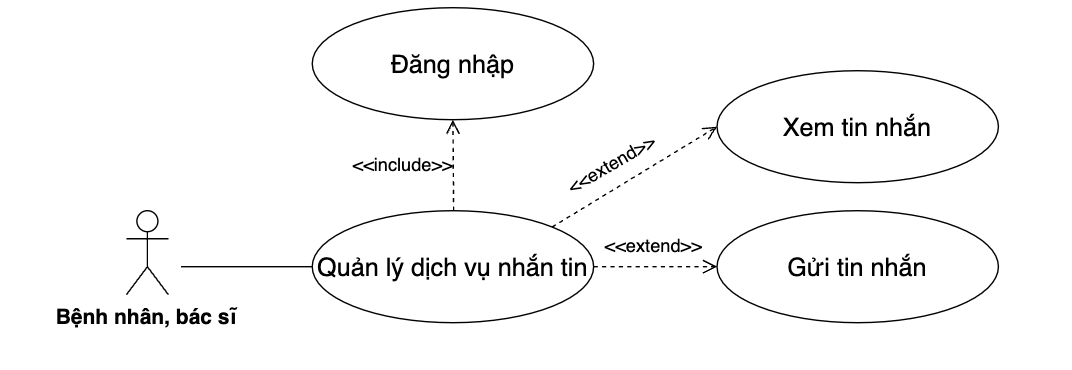
\includegraphics[width=15cm,height=6cm]{Images/mobile_app/use_case_send_receive_message.png}
    \caption[Sơ đồ tuần tự chức năng đăng ký trên App]{\bfseries \fontsize{12pt}{0pt}
    \selectfont Sơ đồ tuần tự chức năng đăng ký trên App}
    \label{hinh21} %đặt tên cho ảnh
  \end{figure}

  \begin{figure}[H]
    \centering
    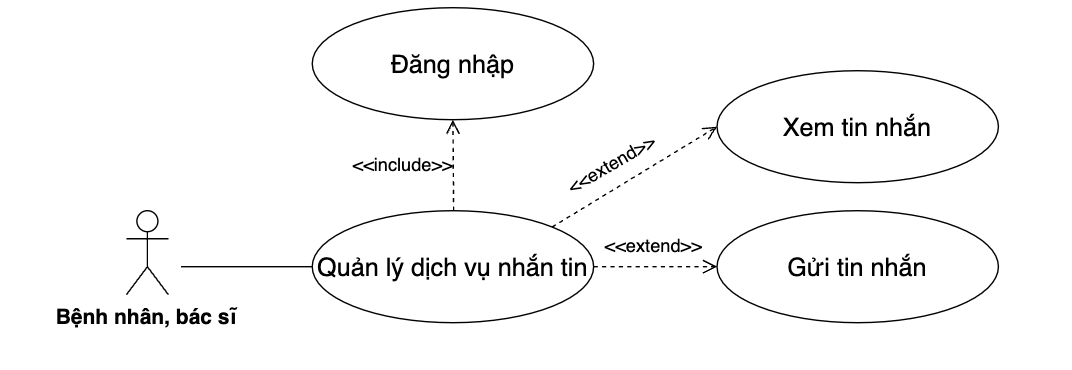
\includegraphics[width=15cm,height=6cm]{Images/mobile_app/use_case_send_receive_message.png}
    \caption[Sơ đồ tuần tự chức năng đăng ký trên App]{\bfseries \fontsize{12pt}{0pt}
    \selectfont Sơ đồ tuần tự chức năng đăng ký trên App}
    \label{hinh21} %đặt tên cho ảnh
  \end{figure}


\subsubsection{Sơ đồ kiến trúc hệ thống}

\begin{figure}[H]
  \centering
  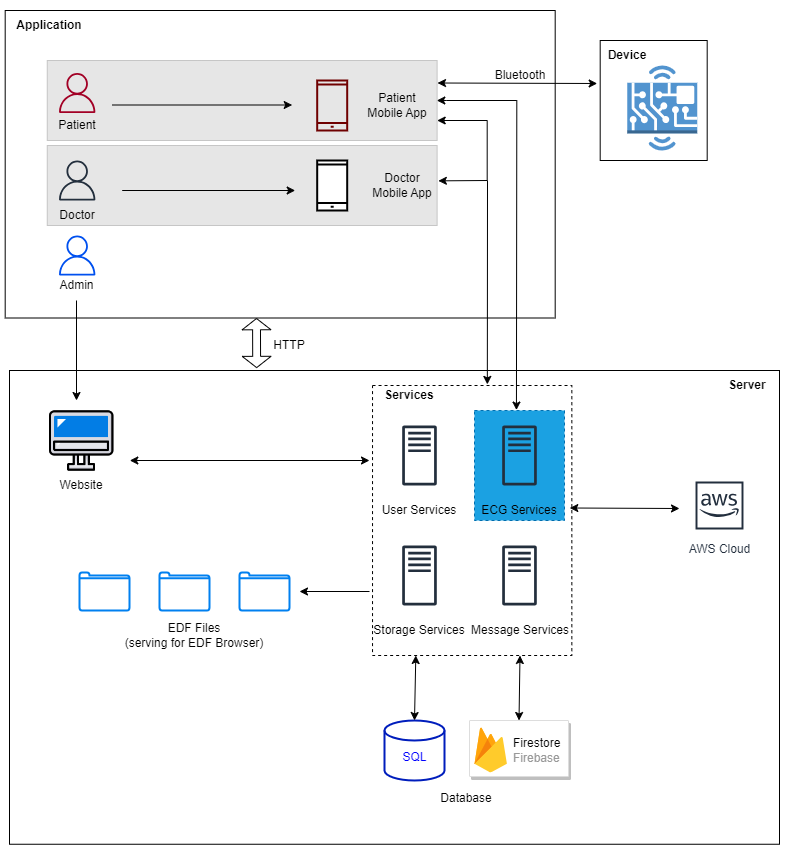
\includegraphics[width=16cm,height=18cm]{Images/system/fmECG_architecture-System Architecture.drawio.png}
  \caption[Kiến trúc hệ thống]{\bfseries \fontsize{12pt}{0pt}\selectfont Kiến trúc hệ thống}
  \label{hinh15} %đặt tên cho ảnh
\end{figure}

\subsubsection{Sơ đồ khối phần mềm}

\paragraph{Ứng dụng cho bệnh nhân}
\mbox{}

\begin{figure}[H]
  \centering
  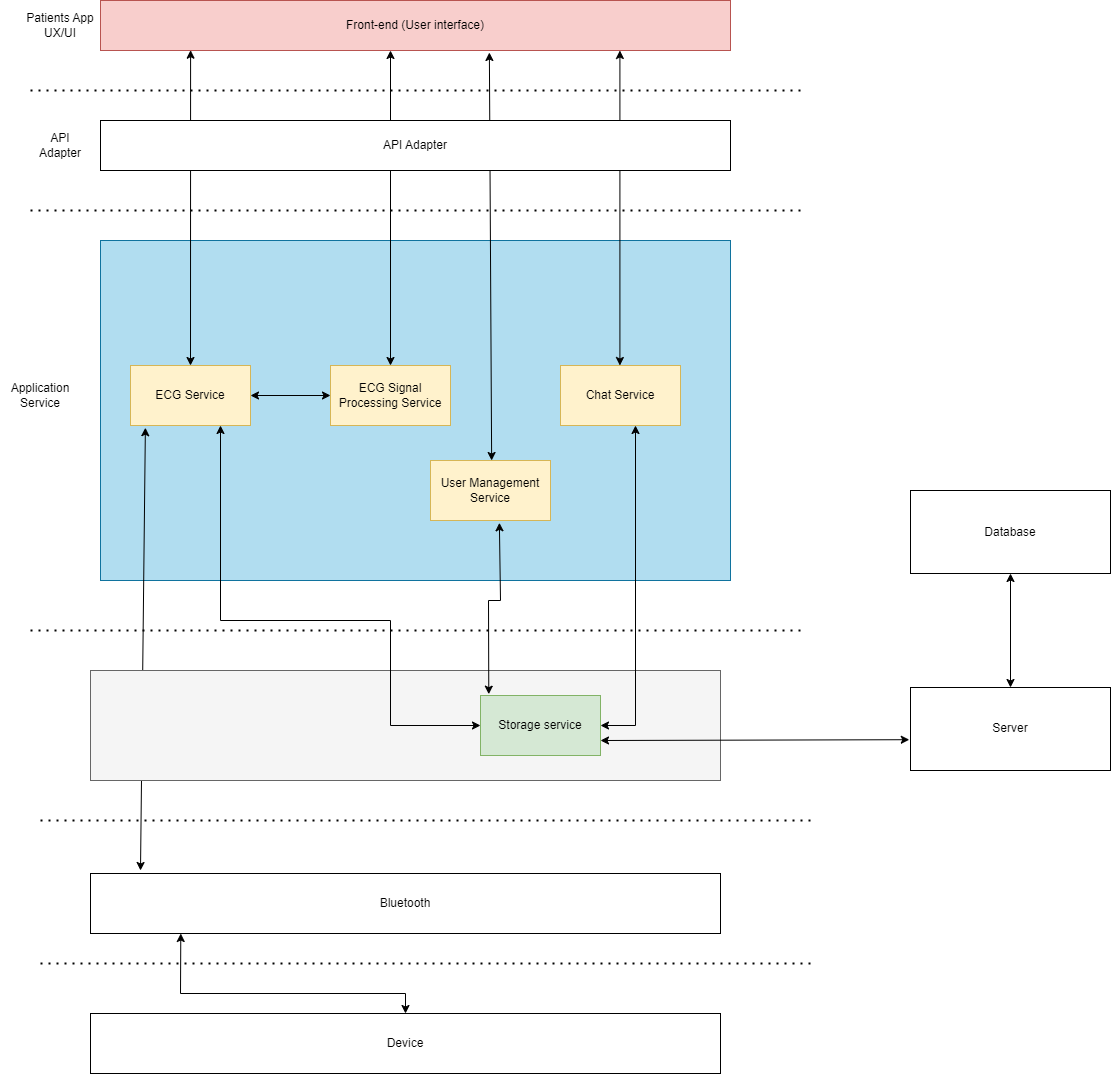
\includegraphics[width=16cm,height=18cm]{Images/system/fmECG_architecture-Patient.drawio.png}
  \caption[Kiến trúc hệ thống]{\bfseries \fontsize{12pt}{0pt}\selectfont Kiến trúc hệ thống}
  \label{hinh15} %đặt tên cho ảnh
\end{figure}

\paragraph{Ứng dụng cho bác sỹ}
\mbox{}


\begin{figure}[H]
  \centering
  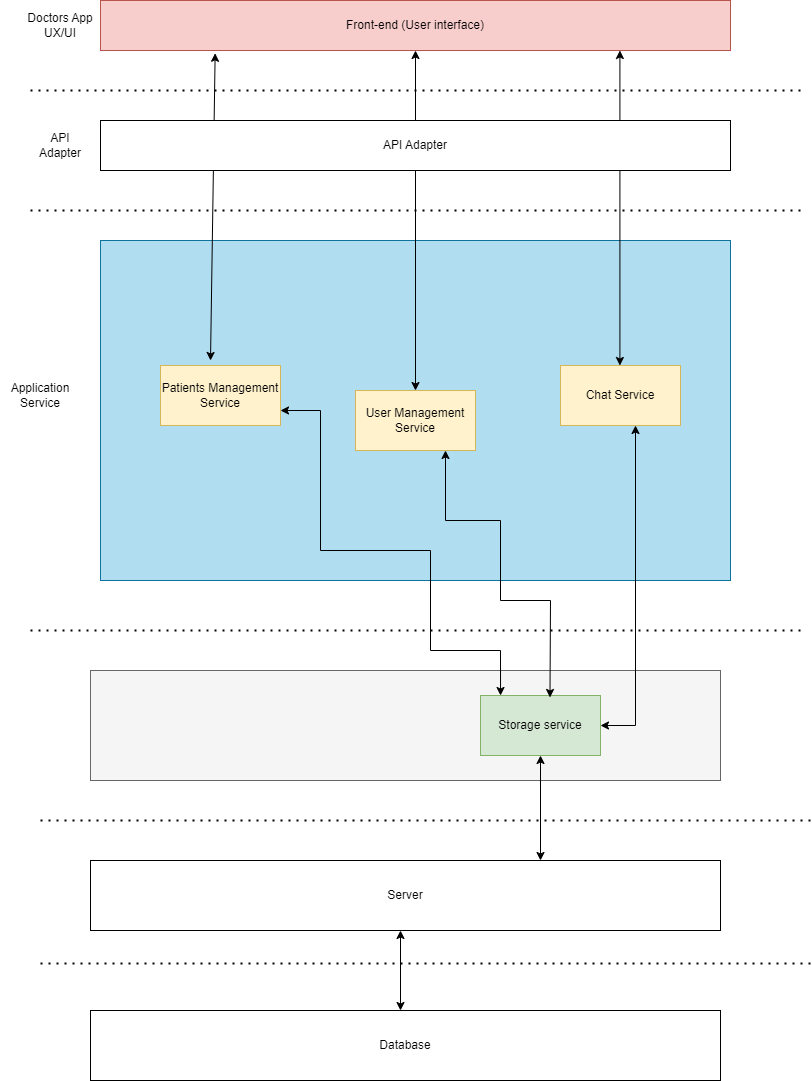
\includegraphics[width=16cm,height=18cm]{Images/system/fmECG_architecture-Doctors.drawio.png}
  \caption[Kiến trúc hệ thống]{\bfseries \fontsize{12pt}{0pt}\selectfont Kiến trúc hệ thống}
  \label{hinh15} %đặt tên cho ảnh
\end{figure}


\paragraph{Website cho admin}
\mbox{}

\begin{figure}[H]
  \centering
  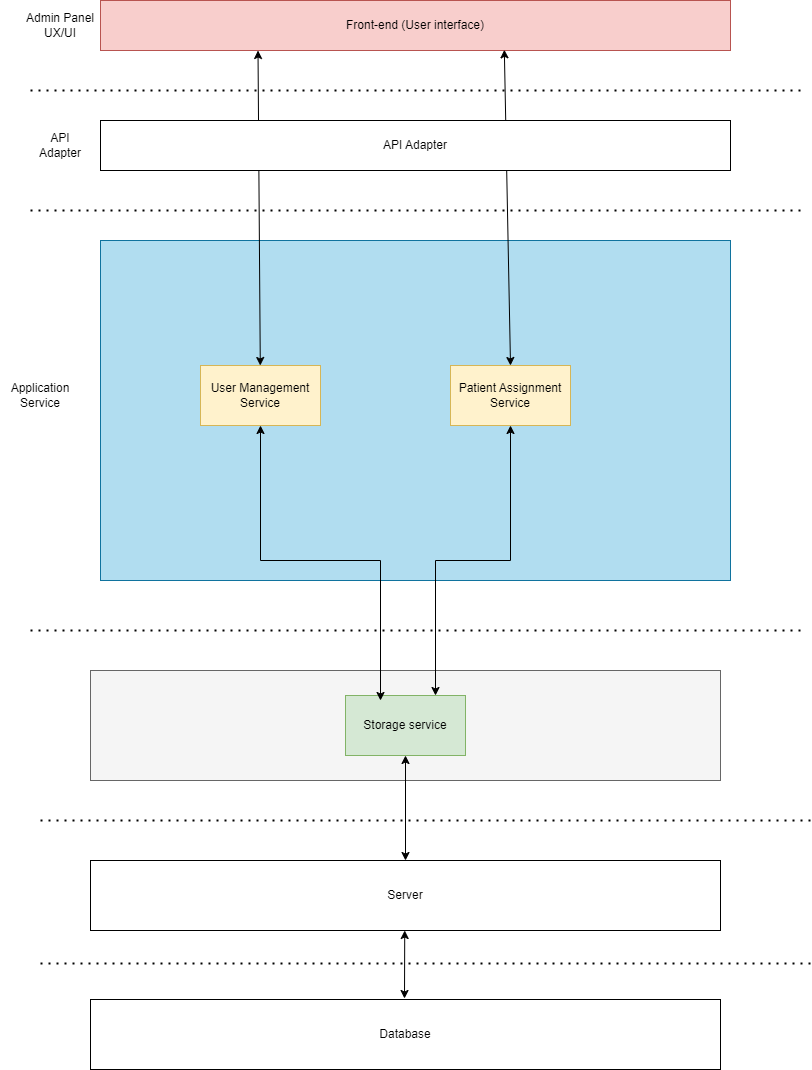
\includegraphics[width=16cm,height=18cm]{Images/system/fmECG_architecture-Admin.drawio.png}
  \caption[Kiến trúc hệ thống]{\bfseries \fontsize{12pt}{0pt}\selectfont Kiến trúc hệ thống}
  \label{hinh15} %đặt tên cho ảnh
\end{figure}

\subsubsection{Sơ đồ tuần tự}

\paragraph{Sơ đồ tuần tự chức năng đăng ký}
\mbox{}

    \begin{figure}[H]
         \centering
         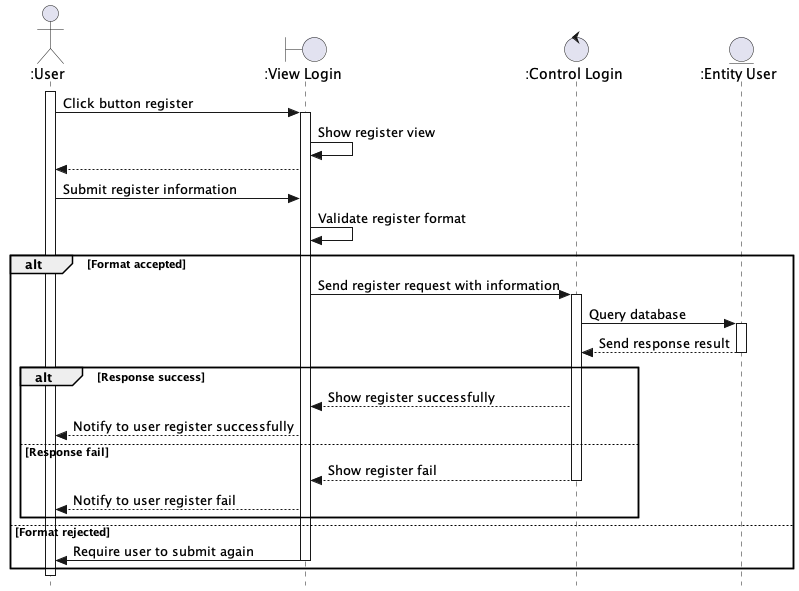
\includegraphics[width=16cm,height=12cm]{Images/mobile_app/register.png}
         \caption[Sơ đồ tuần tự chức năng đăng ký trên App]{\bfseries \fontsize{12pt}{0pt}
         \selectfont Sơ đồ tuần tự chức năng đăng ký trên App}
         \label{hinh21} %đặt tên cho ảnh
    \end{figure}

\paragraph{Sơ đồ tuần tự chức năng đăng nhập}
\mbox{}

    \begin{figure}[H]
         \centering
         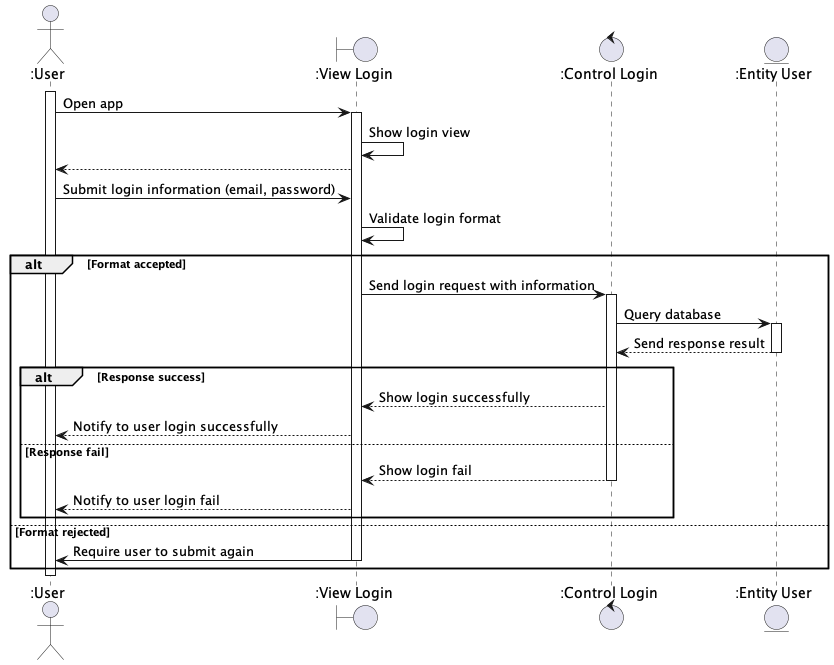
\includegraphics[width=16cm,height=12cm]{Images/mobile_app/login.png}
         \caption[Sơ đồ tuần tự chức năng đăng nhập trên App]{\bfseries \fontsize{12pt}{0pt}
         \selectfont Sơ đồ tuần tự chức năng đăng nhập trên App}
         \label{hinh21} %đặt tên cho ảnh
    \end{figure}

\paragraph{Sơ đồ tuần tự chức năng quên mật khẩu}
\mbox{}

    \begin{figure}[H]
         \centering
         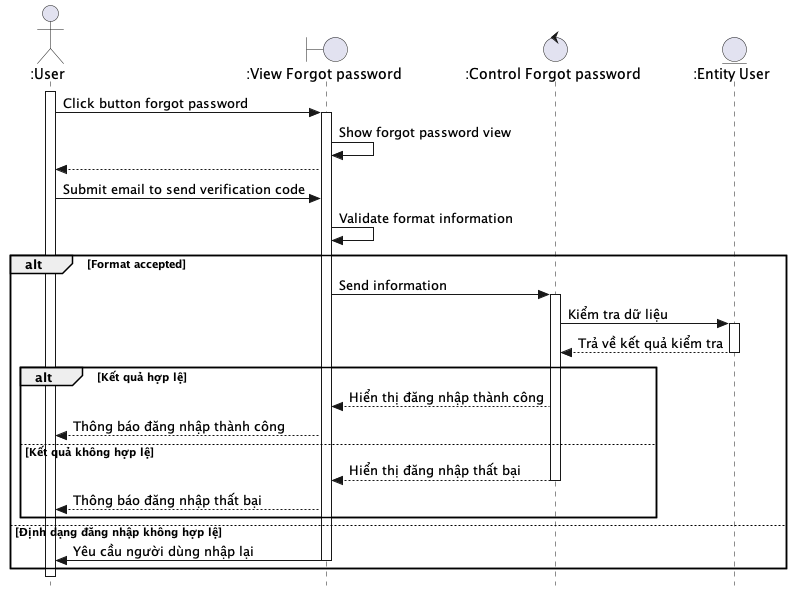
\includegraphics[width=16cm,height=12cm]{Images/mobile_app/forgot_password.png}
         \caption[Sơ đồ tuần tự chức năng quên mật khẩu trên App]{\bfseries \fontsize{12pt}{0pt}
         \selectfont Sơ đồ tuần tự chức năng quên mật khẩu trên App}
         \label{hinh21} %đặt tên cho ảnh
    \end{figure}

\paragraph{Sơ đồ tuần tự chức năng xem lịch sử các lần đo}
\mbox{}


    \begin{figure}[H]
         \centering
         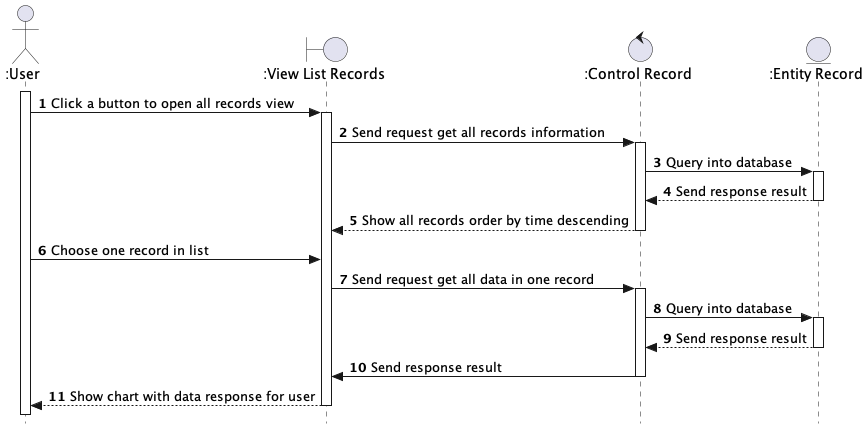
\includegraphics[width=16cm,height=11cm]{Images/mobile_app/view_record_timeline.png}
         \caption[Sơ đồ tuần tự chức năng xem lịch sử các lần đo trên App]{\bfseries \fontsize{12pt}{0pt}
         \selectfont Sơ đồ tuần tự chức năng xem lịch sử các lần đo trên App}
         \label{hinh21} %đặt tên cho ảnh
    \end{figure}

\paragraph{Sơ đồ tuần tự chức năng xem thay đổi thông tin cá nhân}
\mbox{}

  \begin{figure}[H]
        \centering
        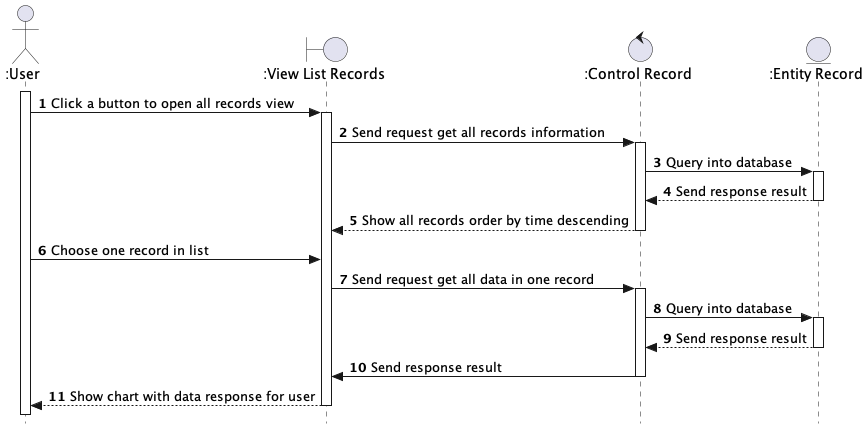
\includegraphics[width=16cm,height=11cm]{Images/mobile_app/view_record_timeline.png}
        \caption[Sơ đồ tuần tự chức năng xem thay đổi thông tin cá nhân trên App]{\bfseries \fontsize{12pt}{0pt}
        \selectfont Sơ đồ tuần tự chức năng xem thay đổi thông tin cá nhân trên App}
        \label{hinh21} %đặt tên cho ảnh
  \end{figure}

  \paragraph{Sơ đồ tuần tự chức năng đổi mật khẩu}
\mbox{}

  \begin{figure}[H]
        \centering
        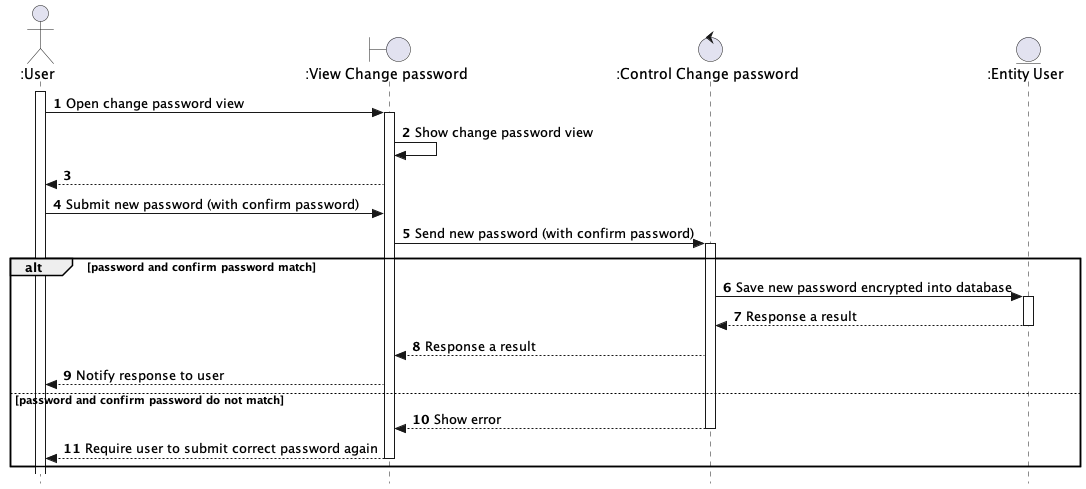
\includegraphics[width=16cm,height=11cm]{Images/mobile_app/change_password.png}
        \caption[Sơ đồ tuần tự chức năng đổi mật khẩu trên App]{\bfseries \fontsize{12pt}{0pt}
        \selectfont Sơ đồ tuần tự chức năng đổi mật khẩu trên App}
        \label{hinh21} %đặt tên cho ảnh
  \end{figure}


\paragraph{Sơ đồ tuần tự chức năng xem/gửi tin nhắn}
\mbox{}

  \begin{figure}[H]
        \centering
        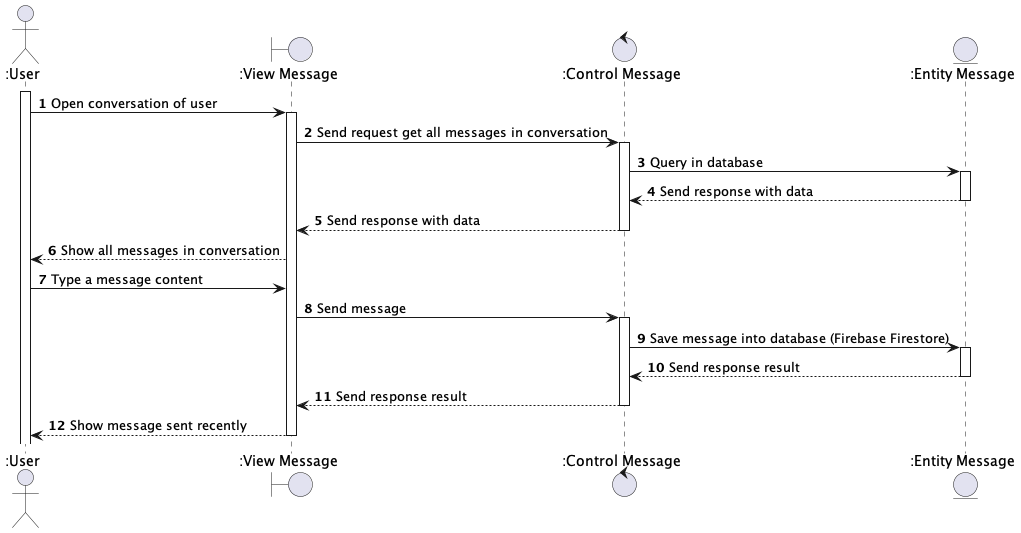
\includegraphics[width=16cm,height=11cm]{Images/mobile_app/send_and_receive_message.png}
        \caption[Sơ đồ tuần tự chức năng xem/gửi tin nhắn trên App]{\bfseries \fontsize{12pt}{0pt}
        \selectfont Sơ đồ tuần tự chức năng xem/gửi tin nhắn trên App}
        \label{hinh21} %đặt tên cho ảnh
  \end{figure}


\paragraph{Sơ đồ tuần tự chức năng xem bài đăng tin tức}
\mbox{}

  \begin{figure}[H]
        \centering
        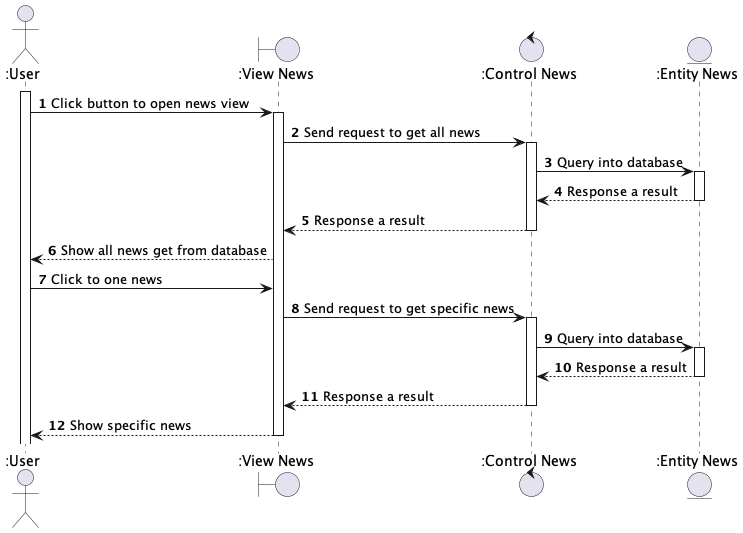
\includegraphics[width=16cm,height=11cm]{Images/mobile_app/view_news.png}
        \caption[ Sơ đồ tuần tự chức năng xem bài đăng tin tứctrên App]{\bfseries \fontsize{12pt}{0pt}
        \selectfont Sơ đồ tuần tự chức năng xem bài đăng tin tức trên App}
        \label{hinh21} %đặt tên cho ảnh
  \end{figure}

\paragraph{Sơ đồ tuần tự chức năng bật/tắt Bluetooth}
\mbox{}

  \begin{figure}[H]
        \centering
        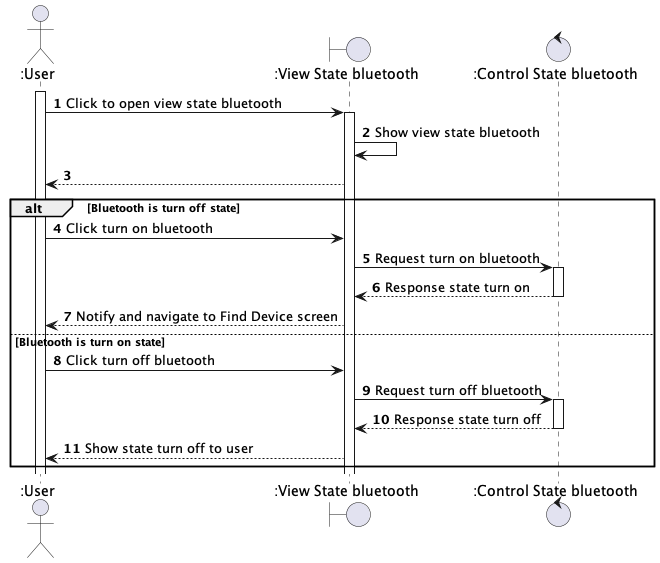
\includegraphics[width=16cm,height=12cm]{Images/mobile_app/turn_on_off_bluetooth.png}
        \caption[Sơ đồ tuần tự chức năng bật/tắt Bluetooth trên App]{\bfseries \fontsize{12pt}{0pt}
        \selectfont Sơ đồ tuần tự chức năng bật/tắt Bluetooth trên App}
        \label{hinh21} %đặt tên cho ảnh
  \end{figure}


\paragraph{Sơ đồ tuần tự chức năng kết nối Bluetooth với thiết bị đo điện tim}
\mbox{}

  \begin{figure}[H]
        \centering
        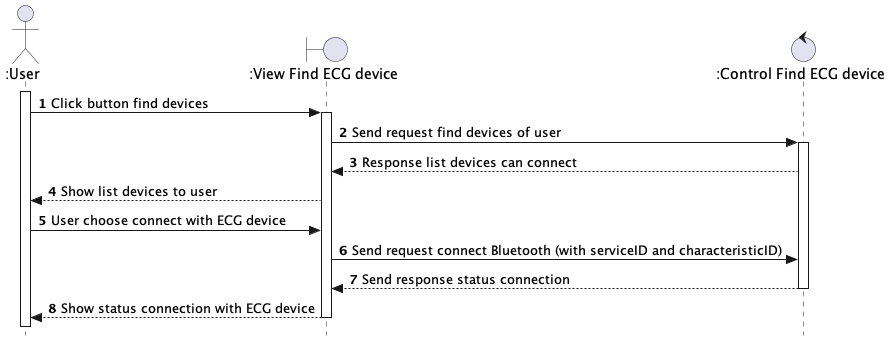
\includegraphics[width=16cm,height=10cm]{Images/mobile_app/connect_with_device.png}
        \caption[Sơ đồ tuần tự chức năng kết nối Bluetooth với thiết bị đo điện tim trên App]{\bfseries \fontsize{12pt}{0pt}
        \selectfont Sơ đồ tuần tự chức năng kết nối Bluetooth với thiết bị đo điện tim trên App}
        \label{hinh21} %đặt tên cho ảnh
  \end{figure}



\paragraph{Sơ đồ tuần tự chức năng ngắt kết nối Bluetooth với thiết bị đo điện tim}
\mbox{}

  \begin{figure}[H]
        \centering
        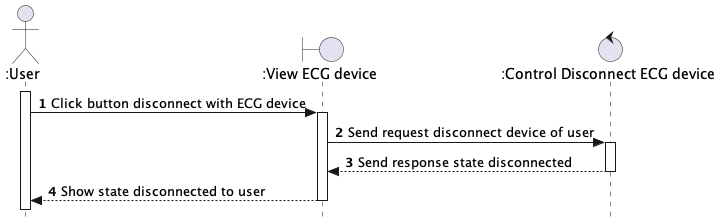
\includegraphics[width=16cm,height=9cm]{Images/mobile_app/disconnect_with_device.png}
        \caption[Sơ đồ tuần tự chức năng ngắt kết nối Bluetooth với thiết bị đo điện tim trên App]{\bfseries \fontsize{12pt}{0pt}
        \selectfont Sơ đồ tuần tự chức năng ngắt kết nối Bluetooth với thiết bị đo điện tim trên App}
        \label{hinh21} %đặt tên cho ảnh
  \end{figure}


\paragraph{Sơ đồ tuần tự chức năng tiến hành đo điện tim}
\mbox{}

  \begin{figure}[H]
        \centering
        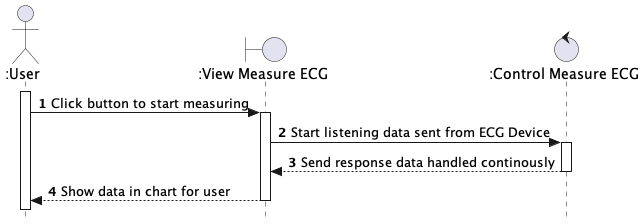
\includegraphics[width=16cm,height=9cm]{Images/mobile_app/start_measuring_ecg.png}
        \caption[Sơ đồ tuần tự chức năng tiến hành đo điện tim trên App]{\bfseries \fontsize{12pt}{0pt}
        \selectfont Sơ đồ tuần tự chức năng tiến hành đo điện tim trên App}
        \label{hinh21} %đặt tên cho ảnh
  \end{figure}
 

\paragraph{Sơ đồ tuần tự chức năng kết thúc quá trình đo điện tim}
\mbox{}

  \begin{figure}[H]
        \centering
        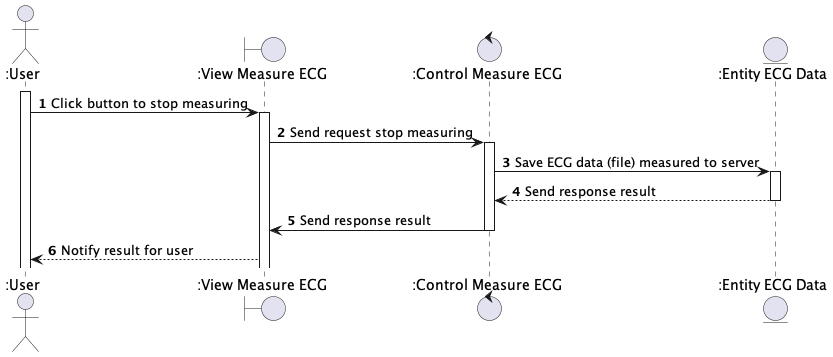
\includegraphics[width=16cm,height=9cm]{Images/mobile_app/end_measuring_ecg.png}
        \caption[Sơ đồ tuần tự chức năng kết thúc quá trình đo điện tim trên App]{\bfseries \fontsize{12pt}{0pt}
        \selectfont Sơ đồ tuần tự chức năng kết thúc quá trình đo điện tim trên App}
        \label{hinh21} %đặt tên cho ảnh
  \end{figure}





\newpage
